%  LaTeX support: latex@mdpi.com 
%  For support, please attach all files needed for compiling as well as the log file, and specify your operating system, LaTeX version, and LaTeX editor.

\newcommand{\qsdauthorname}{Michael Bush}
\newcommand{\qsdauthorinitials}{M.B.}
\newcommand{\qsdauthoremail}{mbush@haddentechnologies.com}
\newcommand{\qsdorcid}{0009-0003-9747-9109}
\newcommand{\qsdcorp}{Hadden Technologies Corporation}
\newcommand{\qsdpapertitle}{The Coherence Envelope: Defining the Minimum Structural Unit of Action in Quantum Substrate Dynamics}

%=================================================================
\documentclass[entropy,article,submit,pdftex,oneauthor]{Definitions/mdpi} 
%\documentclass[preprints,article,submit,pdftex,moreauthors]{Definitions/mdpi} 
% For posting an early version of this manuscript as a preprint, you may use "preprints" as the journal. Changing "submit" to "accept" before posting will remove line numbers.

% Below journals will use APA reference format:
% admsci, aieduc, behavsci, businesses, econometrics, economies, education, ejihpe, famsci, games, humans, ijcs, ijfs, journalmedia, jrfm, languages, psycholint, publications, tourismhosp, youth

% Below journals will use Chicago reference format:
% arts, genealogy, histories, humanities, jintelligence, laws, literature, religions, risks, socsci

%--------------------
% Class Options:
%--------------------
%----------
% journal
%----------
% Choose between the following MDPI journals:
% accountaudit, acoustics, actuators, addictions, adhesives, admsci, adolescents, aerobiology, aerospace, agriculture, agriengineering, agrochemicals, agronomy, ai, air, algorithms, allergies, alloys, amh, analytica, analytics, anatomia, anesthres, animals, antibiotics, antibodies, antioxidants, applbiosci, appliedchem, appliedmath, appliedphys, applmech, applmicrobiol, applnano, applsci, aquacj, architecture, arm, arthropoda, arts, asc, asi, astronomy, atmosphere, atoms, audiolres, automation, axioms, bacteria, batteries, bdcc, behavsci, beverages, biochem, bioengineering, biologics, biology, biomass, biomechanics, biomed, biomedicines, biomedinformatics, biomimetics, biomolecules, biophysica, biosensors, biosphere, biotech, birds, blockchains, bloods, blsf, brainsci, breath, buildings, businesses, cancers, carbon, cardiogenetics, catalysts, cells, ceramics, challenges, chemengineering, chemistry, chemosensors, chemproc, children, chips, cimb, civileng, cleantechnol, climate, clinbioenerg, clinpract, clockssleep, cmd, cmtr, coasts, coatings, colloids, colorants, commodities, complications, compounds, computation, computers, condensedmatter, conservation, constrmater, cosmetics, covid, crops, cryo, cryptography, crystals, csmf, ctn, curroncol, cyber, dairy, data, ddc, dentistry, dermato, dermatopathology, designs, devices, diabetology, diagnostics, dietetics, digital, disabilities, diseases, diversity, dna, drones, dynamics, earth, ebj, ecm, ecologies, econometrics, economies, education, eesp, ejihpe, electricity, electrochem, electronicmat, electronics, encyclopedia, endocrines, energies, eng, engproc, ent, entomology, entropy, environments, epidemiologia, epigenomes, esa, est, famsci, fermentation, fibers, fintech, fire, fishes, fluids, foods, forecasting, forensicsci, forests, fossstud, foundations, fractalfract, fuels, future, futureinternet, futureparasites, futurepharmacol, futurephys, futuretransp, galaxies, games, gases, gastroent, gastrointestdisord, gastronomy, gels, genealogy, genes, geographies, geohazards, geomatics, geometry, geosciences, geotechnics, geriatrics, glacies, grasses, greenhealth, gucdd, hardware, hazardousmatters, healthcare, hearts, hemato, hematolrep, heritage, higheredu, highthroughput, histories, horticulturae, hospitals, humanities, humans, hydrobiology, hydrogen, hydrology, hygiene, idr, iic, ijerph, ijfs, ijgi, ijmd, ijms, ijns, ijpb, ijt, ijtm, ijtpp, ime, immuno, informatics, information, infrastructures, inorganics, insects, instruments, inventions, iot, j, jal, jcdd, jcm, jcp, jcs, jcto, jdad, jdb, jeta, jfb, jfmk, jimaging, jintelligence, jlpea, jmahp, jmmp, jmms, jmp, jmse, jne, jnt, jof, joitmc, joma, jop, jor, journalmedia, jox, jpbi, jpm, jrfm, jsan, jtaer, jvd, jzbg, kidney, kidneydial, kinasesphosphatases, knowledge, labmed, laboratories, land, languages, laws, life, lights, limnolrev, lipidology, liquids, literature, livers, logics, logistics, lubricants, lymphatics, machines, macromol, magnetism, magnetochemistry, make, marinedrugs, materials, materproc, mathematics, mca, measurements, medicina, medicines, medsci, membranes, merits, metabolites, metals, meteorology, methane, metrics, metrology, micro, microarrays, microbiolres, microelectronics, micromachines, microorganisms, microplastics, microwave, minerals, mining, mmphys, modelling, molbank, molecules, mps, msf, mti, multimedia, muscles, nanoenergyadv, nanomanufacturing, nanomaterials, ncrna, ndt, network, neuroglia, neurolint, neurosci, nitrogen, notspecified, nursrep, nutraceuticals, nutrients, obesities, oceans, ohbm, onco, oncopathology, optics, oral, organics, organoids, osteology, oxygen, parasites, parasitologia, particles, pathogens, pathophysiology, pediatrrep, pets, pharmaceuticals, pharmaceutics, pharmacoepidemiology, pharmacy, philosophies, photochem, photonics, phycology, physchem, physics, physiologia, plants, plasma, platforms, pollutants, polymers, polysaccharides, populations, poultry, powders, preprints, proceedings, processes, prosthesis, proteomes, psf, psych, psychiatryint, psychoactives, psycholint, publications, purification, quantumrep, quaternary, qubs, radiation, reactions, realestate, receptors, recycling, regeneration, religions, remotesensing, reports, reprodmed, resources, rheumato, risks, robotics, rsee, ruminants, safety, sci, scipharm, sclerosis, seeds, sensors, separations, sexes, signals, sinusitis, siuj, skins, smartcities, sna, societies, socsci, software, soilsystems, solar, solids, spectroscj, sports, standards, stats, std, stresses, surfaces, surgeries, suschem, sustainability, symmetry, synbio, systems, tae, targets, taxonomy, technologies, telecom, test, textiles, thalassrep, therapeutics, thermo, timespace, tomography, tourismhosp, toxics, toxins, transplantology, transportation, traumacare, traumas, tropicalmed, universe, urbansci, uro, vaccines, vehicles, venereology, vetsci, vibration, virtualworlds, viruses, vision, waste, water, wem, wevj, wild, wind, women, world, youth, zoonoticdis

%---------
% article
%---------
% The default type of manuscript is "article", but can be replaced by: 
% abstract, addendum, article, benchmark, book, bookreview, briefcommunication, briefreport, casereport, changes, clinicopathologicalchallenge, comment, commentary, communication, conceptpaper, conferenceproceedings, correction, conferencereport, creative, datadescriptor, discussion, entry, expressionofconcern, extendedabstract, editorial, essay, erratum, fieldguide, hypothesis, interestingimages, letter, meetingreport, monograph, newbookreceived, obituary, opinion, proceedingpaper, projectreport, reply, retraction, review, perspective, protocol, shortnote, studyprotocol, supfile, systematicreview, technicalnote, viewpoint, guidelines, registeredreport, tutorial,  giantsinurology, urologyaroundtheworld
% supfile = supplementary materials

%----------
% submit
%----------
% The class option "submit" will be changed to "accept" by the Editorial Office when the paper is accepted. This will only make changes to the frontpage (e.g., the logo of the journal will get visible), the headings, and the copyright information. Also, line numbering will be removed. Journal info and pagination for accepted papers will also be assigned by the Editorial Office.

%------------------
% moreauthors
%------------------
% If there is only one author the class option oneauthor should be used. Otherwise use the class option moreauthors.

%---------
% pdftex
%---------
% The option pdftex is for use with pdfLaTeX. Remove "pdftex" for (1) compiling with LaTeX & dvi2pdf (if eps figures are used) or for (2) compiling with XeLaTeX.

%=================================================================
% MDPI internal commands - do not modify
\firstpage{1} 
\makeatletter 
\setcounter{page}{\@firstpage} 
\makeatother
\pubvolume{1}
\issuenum{1}
\articlenumber{0}
\pubyear{2025}
\copyrightyear{2025}
%\externaleditor{Firstname Lastname} % More than 1 editor, please add `` and '' before the last editor name
\datereceived{ } 
\daterevised{ } % Comment out if no revised date
\dateaccepted{ } 
\datepublished{ } 
%\datecorrected{} % For corrected papers: "Corrected: XXX" date in the original paper.
%\dateretracted{} % For retracted papers: "Retracted: XXX" date in the original paper.
\hreflink{https://doi.org/} % If needed use \linebreak
%\doinum{}
%\pdfoutput=1 % Uncommented for upload to arXiv.org
%\CorrStatement{yes}  % For updates
%\longauthorlist{yes} % For many authors that exceed the left citation part

%=================================================================
% Add packages and commands here. The following packages are loaded in our class file: fontenc, inputenc, calc, indentfirst, fancyhdr, graphicx, epstopdf, lastpage, ifthen, float, amsmath, amssymb, lineno, setspace, enumitem, mathpazo, booktabs, titlesec, etoolbox, tabto, xcolor, colortbl, soul, multirow, microtype, tikz, totcount, changepage, attrib, upgreek, array, tabularx, pbox, ragged2e, tocloft, marginnote, marginfix, enotez, amsthm, natbib, hyperref, cleveref, scrextend, url, geometry, newfloat, caption, draftwatermark, seqsplit
% cleveref: load \crefname definitions after \begin{document}

\usepackage{tikz}
\usetikzlibrary{angles, quotes}
\usepackage{pgfplots}
\pgfplotsset{compat=1.17}

%=================================================================
% Please use the following mathematics environments: Theorem, Lemma, Corollary, Proposition, Characterization, Property, Problem, Example, ExamplesandDefinitions, Hypothesis, Remark, Definition, Notation, Assumption
%% For proofs, please use the proof environment (the amsthm package is loaded by the MDPI class).

%=================================================================
% Full title of the paper (Capitalized)
\Title{\qsdpapertitle}


% MDPI internal command: Title for citation in the left column
\TitleCitation{Title}

% Author Orchid ID: enter ID or remove command
\newcommand{\orcidauthorA}{\qsdorcid} % Add \orcidA{} behind the author's name
%\newcommand{\orcidauthorB}{0000-0000-0000-000X} % Add \orcidB{} behind the author's name

% Authors, for the paper (add full first names)
\Author{\qsdauthorname $^{1}$\orcidA{}}

%\longauthorlist{yes}

% MDPI internal command: Authors, for metadata in PDF
\AuthorNames{\qsdauthorname}

% MDPI internal command: Authors, for citation in the left column, only choose below one of them according to the journal style
% If this is a Chicago style journal 
% (arts, genealogy, histories, humanities, jintelligence, laws, literature, religions, risks, socsci): 
% Lastname, Firstname, Firstname Lastname, and Firstname Lastname.

% If this is a APA style journal 
% (admsci, behavsci, businesses, econometrics, economies, education, ejihpe, games, humans, ijfs, journalmedia, jrfm, languages, psycholint, publications, tourismhosp, youth): 
% Lastname, F., Lastname, F., \& Lastname, F.

% If this is a ACS style journal (Except for the above Chicago and APA journals, all others are in the ACS format): 
% Lastname, F.; Lastname, F.; Lastname, F.
\isAPAStyle{%
       \AuthorCitation{Lastname, F., Lastname, F., \& Lastname, F.}
         }{%
        \isChicagoStyle{%
        \AuthorCitation{Lastname, Firstname, Firstname Lastname, and Firstname Lastname.}
        }{
        \AuthorCitation{Lastname, F.; Lastname, F.; Lastname, F.}
        }
}

% Affiliations / Addresses (Add [1] after \address if there is only one affiliation.)
\address{%
$^{1}$ \quad \qsdcorp; \qsdauthoremail\\
%$^{2}$ \quad Affiliation 2; e-mail@e-mail.com
}

% Contact information of the corresponding author
\corres{Correspondence: \qsdauthoremail (\qsdauthorinitials)}

% Current address and/or shared authorship
%\firstnote{Shiloh, IL: Independent Researcher.}  % Current address should not be the same as any items in the Affiliation section.
%\secondnote{These authors contributed equally to this work.}
% The commands \thirdnote{} till \eighthnote{} are available for further notes

%\simplesumm{} % Simple summary

%\conference{} % An extended version of a conference paper


% Abstract (Do not insert blank lines, i.e. \\) 
\abstract{The coherence support scale, \texorpdfstring{\( L_{\text{coh}} \)}{Lcoh}, defines the foundational unit of structure in Quantum Substrate Dynamics (QSD), governing when and how energy, mass, and radiation emerge from a Lorentz-invariant substrate. We define the \texorpdfstring{\( L_{\text{coh}}^3 \)}{Lcoh\^{}3} envelope as the minimum volumetric region required to support a stable, phase-locked mass-phase structure. This coherence boundary sets the conditions for quantized action, scalar recovery, and inertial behavior.
\\
Planck’s constant \texorpdfstring{\( \hbar \)}{hbar} arises structurally from transverse coherence throughput, scalar collapse velocity, and the support area via \texorpdfstring{\( \hbar = \frac{c_t^4}{c_s} \cdot \frac{L_{\text{coh}}^2}{G} \)}{hbar = (ct\^{}4 / cs) * (Lcoh\^{}2 / G)}, 
reframing quantization as a geometric offload condition. Inertia is shown to reflect the cost of reconfiguring all locked envelopes during acceleration, while inertial lag emerges from scalar pacing constraints.
\\
Spectral emissions from mass-phase collapse are serialized by scalar pacing and reflect internal waveform geometry. Stability further requires internal symmetry, providing a structural origin for symmetry in quantum field theory.
\\
In this framework, \texorpdfstring{\( L_{\text{coh}} \)}{Lcoh} defines the substrate’s minimal condition for coherent emergence. Time, mass, inertia, and radiation are not postulates—but outcomes of substrate structure and recovery dynamics.}

% Keywords
\keyword{Quantum Substrate Dynamics; coherence envelope; structural quantization; scalar pacing; Planck constant; mass-phase structure; spectral emission} 

% The fields PACS, MSC, and JEL may be left empty or commented out if not applicable
%\PACS{J0101}
%\MSC{}
%\JEL{}

%%%%%%%%%%%%%%%%%%%%%%%%%%%%%%%%%%%%%%%%%%
% Only for the journal Diversity
%\LSID{\url{http://}}

%%%%%%%%%%%%%%%%%%%%%%%%%%%%%%%%%%%%%%%%%%
% Only for the journal Applied Sciences
%\featuredapplication{Authors are encouraged to provide a concise description of the specific application or a potential application of the work. This section is not mandatory.}
%%%%%%%%%%%%%%%%%%%%%%%%%%%%%%%%%%%%%%%%%%

%%%%%%%%%%%%%%%%%%%%%%%%%%%%%%%%%%%%%%%%%%
% Only for the journal Data
%\dataset{DOI number or link to the deposited data set if the data set is published separately. If the data set shall be published as a supplement to this paper, this field will be filled by the journal editors. In this case, please submit the data set as a supplement.}
%\datasetlicense{License under which the data set is made available (CC0, CC-BY, CC-BY-SA, CC-BY-NC, etc.)}

%%%%%%%%%%%%%%%%%%%%%%%%%%%%%%%%%%%%%%%%%%
% Only for the journal BioTech, Fishes, Neuroimaging and Toxins
%\keycontribution{The breakthroughs or highlights of the manuscript. Authors can write one or two sentences to describe the most important part of the paper.}

%%%%%%%%%%%%%%%%%%%%%%%%%%%%%%%%%%%%%%%%%%
% Only for the journal Encyclopedia
%\encyclopediadef{For entry manuscripts only: please provide a brief overview of the entry title instead of an abstract.}

%%%%%%%%%%%%%%%%%%%%%%%%%%%%%%%%%%%%%%%%%%
% Only for the journal Advances in Respiratory Medicine, Future, Sensors and Smart Cities
%\addhighlights{yes}
%\renewcommand{\addhighlights}{%
%
%\noindent This is an obligatory section in ``Advances in Respiratory Medicine'', ``Future'', ``Sensors'' and ``Smart Cities”, whose goal is to increase the discoverability and readability of the article via search engines and other scholars. Highlights should not be a copy of the abstract, but a simple text allowing the reader to quickly and simplified find out what the article is about and what can be cited from it. Each of these parts should be devoted up to 2~bullet points.\vspace{3pt}\\
%\textbf{What are the main findings?}
% \begin{itemize}[labelsep=2.5mm,topsep=-3pt]
% \item First bullet.
% \item Second bullet.
% \end{itemize}\vspace{3pt}
%\textbf{What is the implication of the main finding?}
% \begin{itemize}[labelsep=2.5mm,topsep=-3pt]
% \item First bullet.
% \item Second bullet.
% \end{itemize}
%}

%%%%%%%%%%%%%%%%%%%%%%%%%%%%%%%%%%%%%%%%%%
\begin{document}
%%%%%%%%%%%%%%%%%%%%%%%%%%%%%%%%%%%%%%%%%%
% The order of the section titles is different for some journals. Please refer to the "Instructions for Authors” on the journal homepage.

%%%%%%%%%%%%%%%%%%%%%%%%%%%%%%%%%%%%%%%%%%
\section{Introduction}
%%%%%%%%%%%%%%%%%%%%%%%%%%%%%%%%%%%%%%%%%%

Planck-scale constants such as \texorpdfstring{\( \hbar \)}{hbar}, \texorpdfstring{\( \ell_P \)}{lP}, and \texorpdfstring{\( E_P \)}{EP} appear throughout modern physics, often demarcating the limits of quantum, relativistic, and gravitational regimes. Yet these constants are typically introduced axiomatically, without physical explanation for why they possess the values they do---or what structural principles enforce their boundaries. Quantization, in particular, is treated as a mathematical feature of operator formalism rather than as a physical outcome of substrate dynamics.

Quantum Substrate Dynamics (QSD)~\cite{bush2025} proposes a coherence-based model of reality in which mass, inertia, and time emerge from the internal behavior of a conserved, Lorentz-invariant substrate. In this framework, mass is not substance but a stable knot of phase-locked coherence; time is not background but the recovery interval between scalar offload events; and energy is not an abstract quantity but the stored and released tension of coherence reconfiguration. Fields, radiation, and force are understood as structured manifestations of wave behavior in this underlying medium, rather than fundamental constructs in their own right.

In such a system, no quantization can occur without structural support. The substrate cannot emit partial wavefronts, support indefinite localization, or transfer energy without geometric coherence. There must exist a minimum spatial domain capable of containing a complete, physically valid offload event---a region over which scalar collapse, transverse propagation, and mass-phase geometry can coexist and reconfigure coherently.

The coherence scale \texorpdfstring{\( L_{\text{coh}} \)}{Lcoh} first appeared in prior work on the structural derivation of Planck’s constant~\cite{bush-planck-2025}, where it emerged as the minimum spatial region required to complete a coherent offload cycle. In that context, it served as a key parameter linking scalar recovery timing, transverse wave propagation, and the substrate’s geometric constraint. However, while it functioned as a derived quantity there, we now recognize \texorpdfstring{\( L_{\text{coh}} \)}{Lcoh} as a physical fundamental in its own right---a boundary condition imposed by the substrate’s structure, not inferred from existing constants.

This paper formalizes that domain: the coherence envelope, denoted \texorpdfstring{\( L_{\text{coh}} \)}{Lcoh}. We show that this envelope defines the substrate’s minimal coherent unit for structured causality. It sets the spatial and temporal scale for quantized action, scalar recovery, and inertial boundary formation within the observable regime of coherent physical emergence. We derive Planck’s constant \texorpdfstring{\( \hbar \)}{hbar} as a function of the substrate’s transverse and scalar propagation modes and this coherence area, and we show how the Planck time and Planck energy emerge directly from this structural constraint. Rather than being imposed limits, these constants are revealed as inevitable outcomes of finite coherence behavior in a physically real medium.

We further explore how phase-locked mass structures within a single \texorpdfstring{\( L_{\text{coh}}^3 \)}{Lcoh\^{}3} envelope exhibit symmetry constraints, spectral signatures, and inertial reconfiguration costs. Stable mass-phase knots must maintain balanced curvature across the full envelope to persist, providing a structural origin for symmetry in quantum field theory. Upon collapse, these knots offload their internal waveform geometry in serialized form, producing characteristic spectral emissions shaped by scalar pacing and bounded by the transverse coherence speed. In this framework, inertia, emission, and quantization all emerge from the same geometric condition: coherence containment within a finite structural volume.

In this sense, \texorpdfstring{\( L_{\text{coh}} \)}{Lcoh} is not just a fundamental length. It is the coherence substrate’s first structural requirement---the boundary condition from which all quantized, radiative, and inertial behavior must follow.

While the structural approach taken here is original to QSD, the questions it addresses have been long-standing in physics. Prior approaches to quantization and field behavior include the standard formalism of quantum field theory~\cite{peskin1995}, symmetry-grounded field construction~\cite{weinberg1995}, and canonical relativistic wave equations~\cite{ryder1996}. Quantum gravity research has pursued minimum length scales and generalized uncertainty relations~\cite{amelino1994, garay1995} as constraints on field behavior near the Planck scale, while condensed matter analogues of spacetime~\cite{volovik2003, barcelo2005} have modeled emergent geometry in coherence-limited media. QSD differs in that it does not assume symmetry or quantization, but derives them from the recoverability conditions of coherent structure within a Lorentz-invariant substrate. The coherence envelope \( L_{\text{coh}}^3 \) offers a physical rather than symbolic constraint, providing the structural foundation on which such phenomena may be consistently modeled and tested.



%%%%%%%%%%%%%%%%%%%%%%%%%%%%%%%%%%%%%%%%%%
\section{Materials and Methods}
%%%%%%%%%%%%%%%%%%%%%%%%%%%%%%%%%%%%%%%%%%
This manuscript was developed through a combination of theoretical derivation, conservation-based modeling, and coherence-structured synthesis. All equations were formulated by the author using first-principles substrate dynamics, with all mathematical expressions derived to maintain causal consistency, empirical validity, and structural compatibility with known relativistic behavior.

In support of the editorial process, generative AI tools—specifically OpenAI's ChatGPT (version GPT-4o, 2025)—were used to assist in:
\begin{itemize}
    \item Generating illustrative figures based on the author’s conceptual framework, with iterative refinement to ensure fidelity to the substrate-based dynamics of the model,
    \item Researching, validating, and cross-referencing related scientific concepts to improve accuracy, contextual alignment, and clarity,
    \item Summarizing and formatting externally sourced material already selected by the author.
\end{itemize}

No original theoretical contributions were generated by the AI system; all scientific claims, hypotheses, derivations, and interpretations were authored and reviewed by the human researcher. The use of ChatGPT is disclosed in alignment with journal policy for transparency in the writing process.

%%%%%%%%%%%%%%%%%%%%%%%%%%%%%%%%%%%%%%%%%%
%\section{Results}

%%%%%%%%%%%%%%%%%%%%%%%%%%%%%%%%%%%%%%%%%%
\section{Discussion}
%%%%%%%%%%%%%%%%%%%%%%%%%%%%%%%%%%%%%%%%%%
\subsection{Quantized Action and the Coherence Envelope}

In conventional quantum mechanics, Planck’s constant \texorpdfstring{\( \hbar \)}{hbar} is introduced axiomatically as the quantization unit of action, governing the minimum scale at which systems transition between discrete energy states. Its physical origin, however, remains unexplained in standard formulations. Within Quantum Substrate Dynamics, \texorpdfstring{\( \hbar \)}{hbar} emerges directly from the internal behavior of the substrate and the structural properties of the coherence envelope.

Specifically, the relation
\[
\hbar = \frac{c_t^4}{c_s} \cdot \frac{L_{\text{coh}}^2}{G}
\]
expresses \texorpdfstring{\( \hbar \)}{hbar} as the product of transverse coherence throughput, scalar collapse pacing, and the minimum spatial area required to support a full offload event. In this formulation, quantized action is not a discrete property of matter or fields, but a geometric and dynamical constraint imposed by the substrate’s coherence mechanics. Action is quantized because the substrate cannot offload partial coherence; it must transfer energy, structure, and phase in complete, self-consistent cycles bounded by \texorpdfstring{\( L_{\text{coh}} \)}{Lcoh} and paced by scalar recovery, see Figure \ref{fig:lcoh}.

\begin{figure}[htbp]
\centering
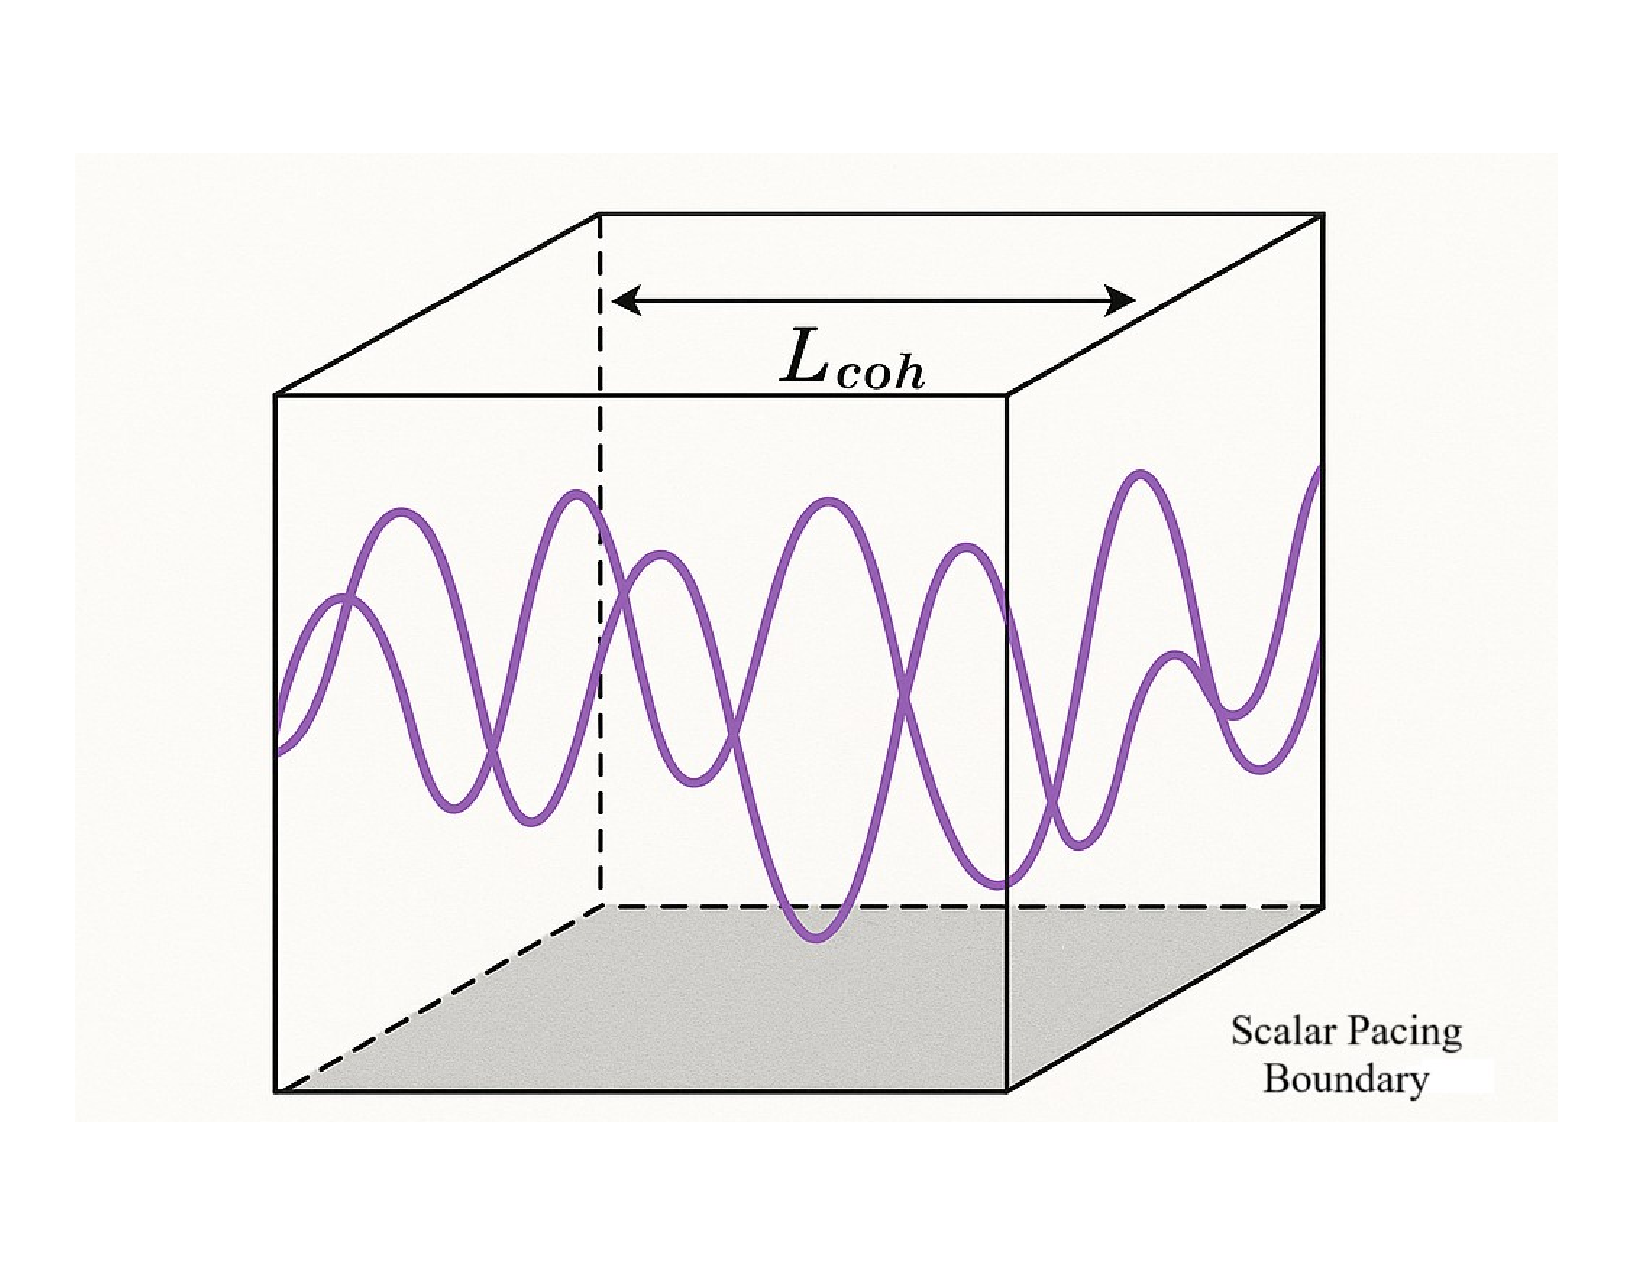
\includegraphics[width=0.85\textwidth]{figures/Lcoh.pdf}
\caption{The coherence envelope \( L_{\text{coh}}^3 \) defines the minimum volume for stable mass-phase structure in QSD. Only phase-closed, curvature-balanced waveforms within this domain can persist or offload. The shaded base marks the scalar pacing boundary.}
\label{fig:lcoh}
\end{figure}

This reinterpretation replaces the mathematical postulate of quantization with a physical process: quantized behavior is a consequence of finite coherence pacing and irreducible structural boundaries. Every quantized transition—whether in atomic spectra, particle decay, or field interaction—can now be seen as a full-envelope reconfiguration event, constrained by the propagation and recovery limits of the substrate. The coherence envelope thus defines not just a spatial unit, but the minimal region within which action can occur, recover, and repeat in a causally consistent manner.
%%%%%%%%%%%%%%%%%%%%%%%%%%%%%%%%%%%%%%%%%
\subsection{Collapse Threshold and Energy Saturation}

While \texorpdfstring{\( \hbar \)}{hbar} defines the minimal coherent action that the substrate can support, the Planck energy \texorpdfstring{\( E_P \)}{Ep} defines the maximal energy that a coherence envelope can contain before collapse becomes inevitable. In QSD, this energy ceiling is not a dimensional artifact but a structural threshold: the point at which stored coherence tension within a single \texorpdfstring{\( L_{\text{coh}}^3 \)}{Lcoh\^{}3} envelope exceeds the substrate’s capacity to maintain stability.

From the QSD framework, Planck energy is derived as
\[
E_P = \frac{c_t^4}{G} \cdot L_{\text{coh}},
\]
which expresses the total energy that can be coherently stored in a single envelope volume before structural failure. This form arises naturally from combining the maximum transverse coherence propagation power (\texorpdfstring{\( c_t^4 \)}{ct\^{}4}), the substrate’s curvature compliance (\texorpdfstring{\( G \)}{G}), and the envelope length scale. Once this threshold is exceeded, the envelope can no longer support internal curvature and phase-locking, and the substrate is forced to respond—either through scalar offload, radiative emission, or coherence rupture.

Collapse in this context is not geometric but structural. The envelope yields because its internal phase configuration can no longer be maintained within the coherence constraints imposed by scalar pacing and transverse coupling. This reframes the Planck energy not as a theoretical limit, but as the energetic saturation point of real coherence structure. Above this point, the substrate cannot store additional energy without breaking symmetry, releasing tension, or initiating new mass-phase formation.

The energy saturation threshold thus defines the boundary between stable containment and dynamic reconfiguration. It is the upper limit of coherent structure, and the inflection point at which offload becomes compulsory.
%%%%%%%%%%%%%%%%%%%%%%%%%%%%%%%%%%%%%%%%%
\subsection{Scalar Recovery and the Pacing of Physical Time}

In QSD, time is not an absolute background or external parameter but a local pacing condition enforced by the substrate’s finite recovery rate. After a coherence envelope undergoes offload—whether through quantized action, radiation, or collapse—it cannot support another offload event until its internal structure has reconfigured and scalar coherence has been restored. This scalar recovery process sets a minimum temporal interval between consecutive events, defining the irreducible pacing of causality.

The Planck time \texorpdfstring{\( t_P \)}{tP} arises directly from this mechanism as
\[
t_P = \frac{L_{\text{coh}}}{c_s},
\]
where \texorpdfstring{\( c_s \)}{cs} is the scalar collapse and recovery velocity. This interval represents the time required for the substrate to fully reconstitute a coherence envelope after a complete offload cycle. No further offload or coherent emission can occur from that region until scalar recovery is complete, regardless of available energy or boundary conditions.

This pacing mechanism provides a structural explanation for temporal quantization and time asymmetry. While transverse propagation can occur at light speed (\texorpdfstring{\( c_t \)}{ct}), scalar recovery introduces a delay that enforces directional flow: energy must offload before recovery, and recovery must complete before the next event. Thus, time flows forward not because of entropy, but because the substrate cannot reverse its recovery process once collapse has occurred.

This view transforms time from a geometric coordinate into a substrate-local constraint—an outcome of coherence behavior rather than a property of spacetime itself. The Planck time is not just a limit of resolution but the intrinsic period of the substrate’s ability to reset and support causally linked phenomena.
%%%%%%%%%%%%%%%%%%%%%%%%%%%%%%%%%%%%%%%%%%
\subsection{Causality, Light Speed, and Transverse Limits}

In relativistic physics, the speed of light is treated as a universal constant and an upper limit on information transfer, but its physical origin remains undefined. In QSD, the transverse coherence speed \texorpdfstring{\( c_t \)}{ct} emerges as a structural limit on how fast energy and phase information can be coherently propagated across the substrate. It represents the maximum transverse throughput available to transfer phase-locked coherence between neighboring regions without loss or distortion.

This transverse limit defines the boundary between coherent communication and structural rupture. Any attempt to transmit energy faster than \texorpdfstring{\( c_t \)}{ct} would violate the substrate's ability to maintain transverse phase continuity, leading to destructive interference, decoherence, or scalar failure modes. As such, \texorpdfstring{\( c_t \)}{ct} is not a postulate, but a derived limit from within the structure of the substrate itself.

Causality in QSD is therefore coherence-limited. Events cannot influence one another unless a coherence envelope can be offloaded and re-established between them. Transverse propagation governs how fast that influence can spread, while scalar pacing governs when such events can reoccur. Together, these two speeds—\texorpdfstring{\( c_t \)}{ct} and \texorpdfstring{\( c_s \)}{cs}—fully define the structure of causal propagation in the substrate.

This framework also clarifies why all observers within their own local frame measure the same speed of light. In QSD, the transverse coherence speed \( c_t \) is not tied to any emitter, receiver, or global reference frame—it is a structural property of the substrate that governs the maximum rate at which coherent information may propagate. As a result, each observer experiences the same causal boundary conditions locally, regardless of motion. What special relativity treats as postulate, QSD interprets as substrate pacing: the invariance of light speed reflects the local coherence limits of the medium, not a geometric symmetry imposed from outside.

%%%%%%%%%%%%%%%%%%%%%%%%%%%%%%%%%%%%%%%%%%
\subsection{Coherence-Limited Observability and Emergence}

While the substrate in QSD may support substructure, fluctuations, or phase variation below the coherence threshold, no quantized, persistent, or causally observable phenomenon can emerge without satisfying the structural conditions imposed by the coherence envelope \texorpdfstring{\( L_{\text{coh}}^3 \)}{Lcoh\^{}3}. In this sense, all measurable physical behavior arises not from the full dynamics of the substrate, but from those coherent configurations that exceed the minimum requirements for stability, recovery, and causal propagation.

Quantized phenomena—mass, radiation, inertia, field effects—only occur when energy and phase can be structured within a bounded region, coherently offloaded, and scalar-recovered in accordance with the envelope’s constraints. Structures smaller than \texorpdfstring{\( L_{\text{coh}} \)}{Lcoh} may exist within the substrate, but they cannot emit, persist, or interact in a way that survives as causal, observable action. The coherence envelope therefore defines the lower bound of physical emergence: the point at which structure becomes recoverable, measurable, and capable of producing reconfigurable effects within the causal field.

This threshold condition reframes classical ideas of point particles or spacetime events as idealizations. No event in QSD can occur without a supporting coherence envelope; no particle can interact without occupying a real structural volume; no signal can propagate without phase continuity. Observation, in this framework, is not a passive sampling of existing states but the registration of complete offload-recovery cycles that meet the substrate’s structural minimum. Below that level, physics remains silent—not because it is empty, but because it cannot yet speak coherently.
%%%%%%%%%%%%%%%%%%%%%%%%%%%%%%%%%%%%%%%%%%
\subsection{Mass-Phase Geometry and Structural Containment}

In QSD, mass is understood not as substance but as a persistent, phase-locked configuration of substrate coherence. For such a mass-phase knot to remain stable, its structure must be fully contained within a coherence envelope \texorpdfstring{\( L_{\text{coh}}^3 \)}{Lcoh\^{}3}, where it can maintain internal tension, curvature balance, and scalar recovery synchrony. This requirement imposes strict geometric and energetic constraints on what constitutes a physically viable mass structure.

The internal waveform of a stable mass-phase must “close” on itself within the envelope, forming a complete, curvature-balanced coherence knot. Partial or asymmetric waveforms cannot maintain coherence under scalar pacing and are either immediately reabsorbed, collapse into scalar emission, or destabilize into multi-envelope extensions. The Planck energy \texorpdfstring{\( E_P = \frac{c_t^4}{G} \cdot L_{\text{coh}} \)}{Ep = (ct\^{}4 / G) * Lcoh} defines the maximum energy that can be stored within a single envelope before collapse is structurally enforced.

These criteria provide a physical basis for mass stability and particle identity. A particle that fits entirely within \texorpdfstring{\( L_{\text{coh}}^3 \)}{Lcoh\^{}3} and satisfies curvature and pacing constraints may persist as a localized, inertial entity. Conversely, high-energy or topologically unstable mass-phase structures must either offload or extend, explaining particle decay, instability, and structural thresholds.

This may offer a coherence-based interpretation for why elements beyond a certain atomic number rapidly decay or fail to remain stable. As the internal waveform of a large nucleus becomes increasingly complex and energetically dense, it may exceed the structural tolerance of a coherent envelope. Such overstuffed configurations could break symmetry, violate scalar pacing, or surpass \( E_P \), forcing the substrate to reject the structure via immediate offload or fragmentation. Heavy element decay, in this view, may reflect the substrate’s inability to sustain mass-phase knots that overfill the geometry of persistence.

This perspective grounds the existence of particles in the substrate’s structural capacity and offers a principled explanation for why only certain mass-phase forms are stable. It connects inertial behavior and structural persistence to real, finite coherence conditions, replacing point-like abstractions with physically meaningful geometry.

%%%%%%%%%%%%%%%%%%%%%%%%%%%%%%%%%%%%%%%%%%
\subsection{Inertial Drag and Scalar-Limited Reconfiguration}
\label{sec:coherent-momentum-quantum}
Inertia, within the QSD framework, arises from the substrate's resistance to reconfiguring a locked mass-phase structure across adjacent coherence envelopes. A stable mass-phase occupies one or more saturated \texorpdfstring{\( L_{\text{coh}}^3 \)}{Lcoh\^{}3} regions, each of which holds internal curvature and phase structure that must remain coherent to preserve mass identity. To accelerate such a structure, the substrate must offload and re-establish the entire configuration in a neighboring envelope, without violating scalar pacing or coherence integrity.

This requirement introduces a real energetic cost: all participating envelopes must reconfigure simultaneously, and scalar recovery must complete before each region can accept or emit new coherence. The resistance to this coordinated offload defines inertial drag. Unlike classical mechanics, where mass resists motion due to unspecified “inertial property,” QSD identifies the physical cause: the substrate’s enforcement of coherence continuity and pacing constraints across structurally saturated regions.

More massive or spatially extended structures involve a greater number of coupled envelopes and thus require more energy to reconfigure. Additionally, complex internal geometry increases the burden of maintaining coherence alignment during movement, further amplifying inertial resistance. In this view, inertia scales with the total structural content of the mass-phase—not simply its energy or rest mass, but its curvature density and coherence volume.

Inertial drag is therefore not a passive property, but a dynamically enforced structural constraint. It emerges directly from the coherence envelope’s resistance to partial reconfiguration, scalar pacing limits, and the cost of preserving internal structure during offload. In QSD, motion is not continuous translation but envelope-wise reconfiguration. As such, the energetic cost of movement is not divisible below the scale of \texorpdfstring{\( L_{\text{coh}}^3 \)}{Lcoh\^{}3}. No partial offload or sub-envelope translation is permitted; a mass-phase structure must fully reconfigure across a coherence boundary to change position.

This introduces a minimum unit of motion and a corresponding irreducible energetic impulse—referred to here as a \textit{coherent momentum quantum}. Unlike conventional momentum, which is treated as continuously variable, QSD suggests that changes in motion occur in discrete, full-envelope transitions governed by structural compliance. The existence of such momentum quanta may offer observable consequences in high-precision force-transfer experiments or coherence-limited systems. Motion is not free; it is structurally earned through substrate compliance, and must be paid for in full at each reconfiguration step.  See Appendix \ref{app:coherent-momentum-quantum}.

%%%%%%%%%%%%%%%%%%%%%%%%%%%%%%%%%%%%%%%%%%
\subsection{Inertial Lag and Coherence Boundary Transitions}

In addition to the energetic cost of reconfiguration, coherent mass-phase structures in QSD experience a temporal delay during acceleration or deceleration. This phenomenon, termed inertial lag, arises from the requirement that all reconfiguration events occur at discrete coherence boundaries defined by the \texorpdfstring{\( L_{\text{coh}}^3 \)}{Lcoh\^{}3} envelope. Because no partial offload is permitted, motion cannot proceed continuously—it must proceed through synchronized transitions across complete coherence volumes.

When a force is applied to change the velocity of a mass-phase knot, the substrate cannot respond instantly. It must first align scalar recovery pacing, internal geometry, and envelope boundary conditions to support coherent reconfiguration. Until these conditions are met, the mass-phase structure persists in its original state. The result is a measurable delay between applied force and structural response, reflecting the time required to complete a valid offload–recover cycle.

This delay becomes more pronounced for larger, denser, or more geometrically complex mass-phase configurations. While the scalar pacing interval \( t_P = \frac{L_{\text{coh}}}{c_s} \) sets the minimum timing constraint for reconfiguration, the actual lag duration increases with the coordination burden required to transition multiple envelopes coherently. Crucially, the substrate enforces an all-or-nothing condition: all coupled envelopes must reconfigure together, and the total energy required for that structural transition must be supplied in full. No partial transitions are permitted, and no motion can begin until coherence integrity and pacing readiness are satisfied across the entire structure.

We model this coherence-aligned delay using a structural complexity factor \( \kappa \), such that
\[
\Delta t_{\text{lag}} = \kappa \cdot t_P,
\]
where \( \kappa \geq 1 \) reflects the geometric complexity, envelope coupling, and internal curvature of the mass-phase configuration. Inertial lag thus scales not only with mass, but with the physical structure of the waveform. QSD reframes it not as a mechanical artifact, but as a substrate-enforced delay condition: motion is permitted only when the entire configuration is structurally ready, causally recoverable, and energetically complete.

%%%%%%%%%%%%%%%%%%%%%%%%%%%%%%%%%%%%%%%%%%
\subsection{Spectral Emission as Serialized Offload Geometry}

When a mass-phase structure confined within an \texorpdfstring{\( L_{\text{coh}}^3 \)}{Lcoh\^{}3} envelope collapses, the offload process does not emit energy as an undifferentiated pulse. Instead, the internal waveform geometry of the coherence knot is released in a serialized, scalar-paced sequence. The resulting spectral signature is not merely a quantum energy transition—it is a physically structured readout of the knot’s internal phase configuration.

In QSD, transverse coherence modes propagate at \texorpdfstring{\( c_t \)}{ct}, while scalar collapse enforces a pacing constraint that limits how quickly energy can be offloaded. These two factors combine to form a substrate-limited serialization channel through which the knot's internal structure is progressively expressed as radiative output. Each spatial mode within the mass-phase waveform contributes a frequency component to the overall spectrum, producing a sequence of emissions that encode the original configuration.

The spectrum that results—whether in atomic transitions, decay cascades, or photon emission—is therefore not abstract or statistical. It is a coherent fingerprint of internal structure, governed by scalar recovery pacing and filtered through transverse propagation constraints. Emitted spectral lines correspond to the curvature modes and nodal features of the original mass-phase geometry, Figure \ref{fig:spectral}.

%\setlength{\abovecaptionskip}{.1cm}
\begin{figure}[htbp]
\centering
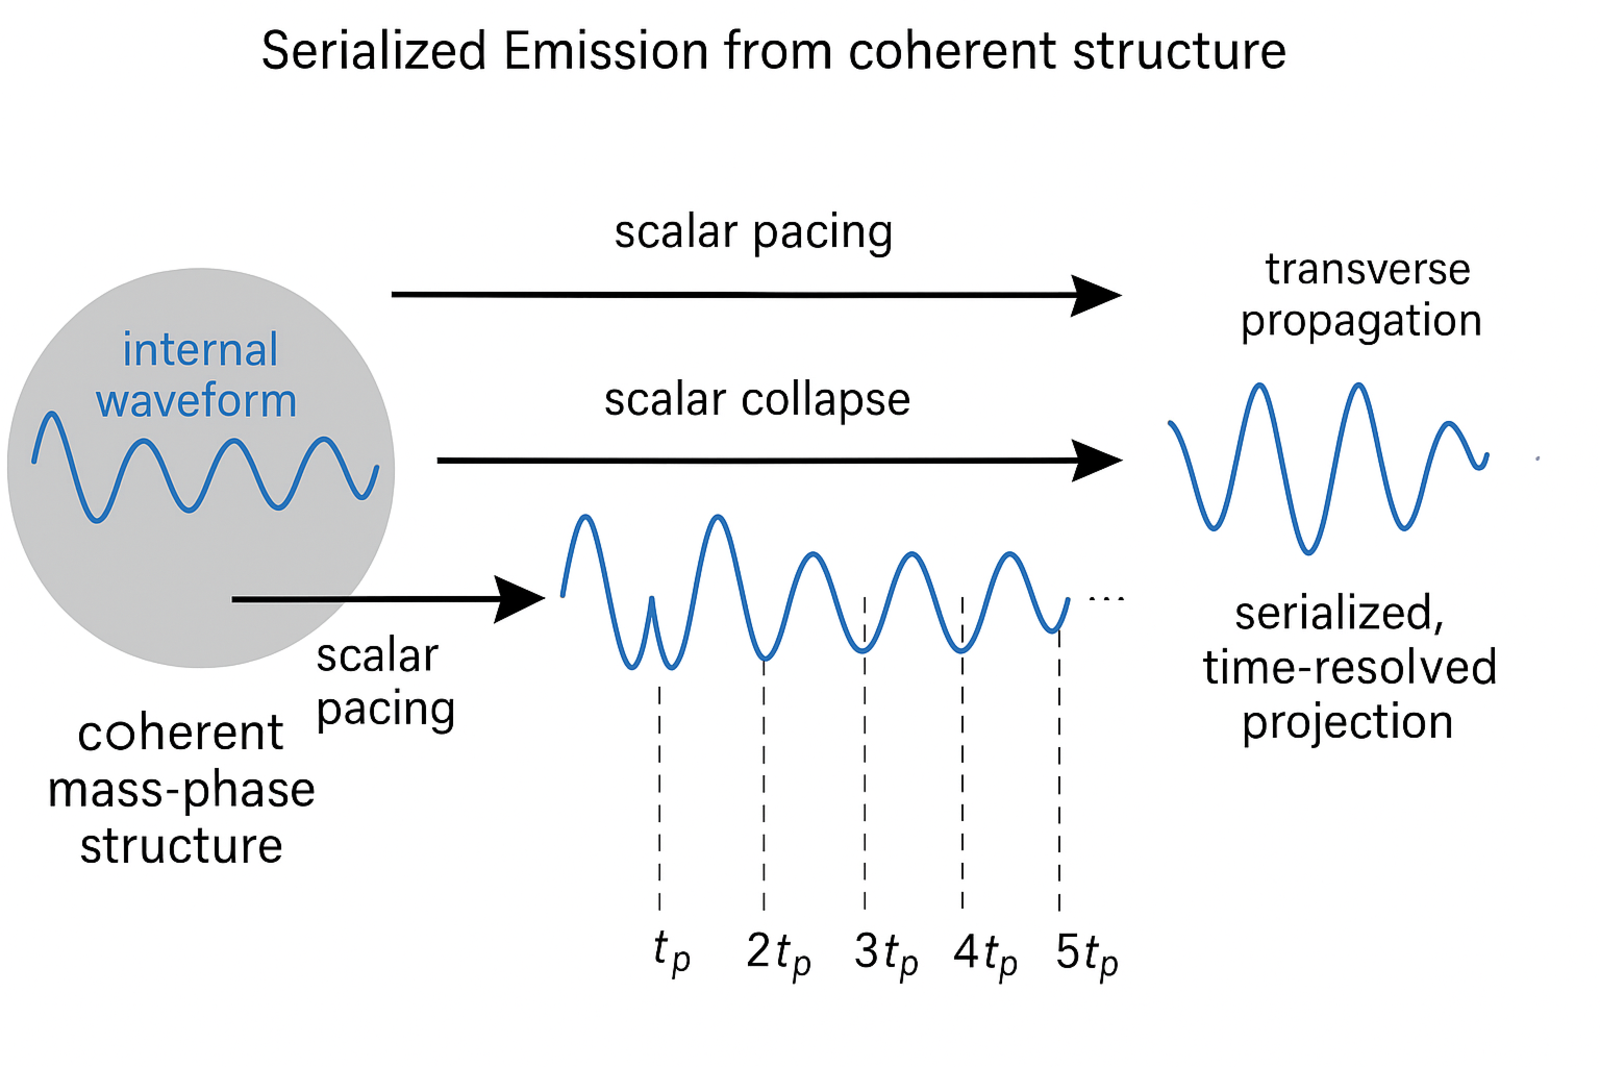
\includegraphics[width=0.85\textwidth]{figures/spectral.pdf}
\caption{Serialized emission from a coherent mass-phase structure in QSD. Internal waveform geometry is offloaded in discrete intervals paced by \( t_p \), producing a time-resolved spectral projection governed by scalar collapse and transverse propagation.}

\label{fig:spectral}
\end{figure}

This serialization of offload explains why spectral lines are stable, reproducible, and discrete: only structures that couple coherently to the substrate’s allowed transverse channels will radiate. Others will collapse as scalar waves or be reabsorbed. QSD thus reframes spectral emission as a real-time projection of internal mass-phase structure, resolved by substrate mechanics into temporally ordered waveforms. Spectroscopy, in this context, becomes an act of waveform retrieval: observing the serialized signature of coherence geometry as it offloads into the causal field.

This behavior can be modeled as a scalar-paced decomposition of the internal waveform. Let the spatial geometry of the mass-phase knot be expressed as a superposition of modes,
\[
\phi(x) = \sum_n A_n \sin(k_n x),
\]
where each mode \( k_n \) corresponds to a curvature or nodal feature of the structure. During collapse, scalar pacing permits offload of these components sequentially, with a delay of one pacing interval \( t_P = \frac{L_{\text{coh}}}{c_s} \) between each. The resulting emitted waveform takes the form
\[
\Psi_{\text{emit}}(t, x) = \sum_n A_n \sin(k_n x) \cdot \Theta(t - n t_P),
\]
where \( \Theta \) is the Heaviside step function representing substrate gating. This simple model illustrates how the spectral output is not simultaneous but serialized—emerging as a time-resolved projection of internal structure, shaped by the knot’s mode content and the substrate’s scalar pacing limit.

While coherence conditions are most generally expressed in Cartesian coordinates to accommodate arbitrary structure, the radial view becomes physically privileged when modeling substrate collapse and emission. In such cases, the coherence envelope acts as a spherical source of serialized energy release, with radial projection into the surrounding substrate. This framing helps explain why offload events often appear as particle-like emissions: the collapse of a coherent mass-phase knot produces a localized, symmetric, temporally gated field signature observable as quantized transfer.

In the case of a spherically symmetric mass-phase knot, the offload process may be modeled as a radial projection of curvature modes emitted outward in scalar-paced intervals. Let the internal structure be expressed in radial coordinates as a sum of spherical modes:
\[
\phi(r) = \sum_n A_n \sin(k_n r),
\]
where \( r \in [0, L_{\text{coh}}] \) and \( k_n \) denotes the radial wave number of each internal mode. During scalar collapse, each mode is offloaded sequentially into the substrate, gated by scalar pacing. The emitted radial wave structure can then be modeled as:
\[
\Psi_{\text{emit}}(r, t) = \sum_n A_n \frac{\sin(k_n r)}{r} \cdot \Theta(t - n t_P),
\]
where \( \Theta \) enforces scalar pacing at interval \( t_P = \frac{L_{\text{coh}}}{c_s} \). The \( \frac{1}{r} \) factor reflects spherical propagation, ensuring energy conservation across expanding shells. This model describes offload not as an instantaneous pulse, but as a serialized radial projection of internal structure—mirroring the quantized, time-resolved spectra observed in particle-like emission events.

In this interpretation, the coherence envelope acts as a spherically collapsing emitter, and what is detected as a discrete "particle" may in fact be the structured output of this paced offload process. QSD thus reinterprets particle detection as localized substrate response to radial collapse, preserving phase structure, temporal order, and transverse coherence throughout.

This behavior parallels known phenomena in mode-locked laser systems~\cite{loudon2000}, where discrete frequencies emerge from temporally structured field emission. Similarly, the QSD framework mirrors mode decomposition strategies used in field theory~\cite{griffiths1995, peskin1995}, but replaces abstract operator transitions with causally enforced scalar pacing. The result is a predictive, substrate-grounded model of spectral emission as serialized coherence geometry.

%%%%%%%%%%%%%%%%%%%%%%%%%%%%%%%%%%
\subsection{Interference and Structural Superposition}
%%%%%%%%%%%%%%%%%%%%%%%%%%%%%%%%%%
In classical wave theory and quantum mechanics, interference is described as the algebraic addition of wave amplitudes—constructive or destructive depending on phase alignment. In QSD, this behavior is reinterpreted structurally: waveforms are not simply summed, but superposed within a coherence envelope \( L_{\text{coh}}^3 \), where they must collectively satisfy curvature, pacing, and closure conditions to initiate causal offload.

Let two incoming waveforms be given by
\[
\phi_1(x, t) = A \sin(kx - \omega t), \quad \phi_2(x, t) = -A \sin(kx - \omega t),
\]
such that their superposition becomes
\[
\phi_{\text{total}}(x, t) = \phi_1 + \phi_2 = 0.
\]
In conventional analysis, this is seen as destructive interference—net amplitude zero. But in QSD, this condition has deeper structural meaning: the combined waveform fails to generate a coherence pattern that satisfies the curvature and pacing requirements for offload within the envelope. There is no valid structure to serialize, and the substrate registers a null event.

This provides a physical mechanism for destructive interference: it is not a loss of energy, but a structural disqualification. Only those superpositions where the total waveform \( \phi_{\text{total}}(x, t) \) satisfies the envelope’s coherence conditions—including net curvature balance,
\[
\int_{L_{\text{coh}}^3} \nabla^2 \phi_{\text{total}} \, d^3x = 0,
\]
and phase closure across boundary domains—can result in causal offload.

From the substrate’s perspective, energy is not a conserved background quantity—it is a byproduct of valid structural offload. If a waveform or superposition fails to meet coherence criteria, no offload occurs and no energy is serialized. The apparent “energy loss” observed in destructive interference is not a disappearance, but a cancellation of causal readiness. There was never any energy to begin with in the classical sense—only incompatible curvature disturbances that nullified each other before serialization. The substrate acts only when permitted by structure.

This substrate-based view does not invalidate the quantum field theoretic formalism that correctly tracks energy and phase statistics. Rather, it reveals the structural origin behind the rules. The Feynman path integral and field operator models~\cite{feynman-qed} faithfully describe outcomes because they are tallying coherent contributions that the substrate ultimately permits. QSD simply adds the underlying reason why such contributions are allowed or denied.

Thus, QSD offers a physical reinterpretation of interference not as a mystical probability effect or wave cancellation, but as a substrate-level coherence filter. A region may contain overlapping wave disturbances, but if the resulting structure fails to form a valid causal entity, the system remains silent. The substrate acts not on energy alone, but on structural integrity—and interference becomes the enforcement of structural exclusion.


%%%%%%%%%%%%%%%%%%%%%%%%%%%%%%%%%%%%%%%%%%
\subsection{Symmetry as a Requirement for Persistence}

In conventional quantum theory, symmetry is a foundational principle: conservation laws, particle classifications, and interaction rules are all derived from assumed invariance under specific transformations. Yet the physical origin of this symmetry is typically taken as axiomatic. In QSD, by contrast, symmetry arises as a structural necessity for coherence stability within a bounded envelope.

For a mass-phase coherence knot to remain locked within a single \texorpdfstring{\( L_{\text{coh}}^3 \)}{Lcoh\^{}3} envelope, its internal waveform geometry must be both curvature-balanced and phase-closed in all three spatial dimensions. This requirement can be expressed through structural conditions that ensure geometric and energetic stability. The waveform must satisfy closure in each spatial dimension:
\[
\phi(x + L_{\text{coh}}, y, z) = \phi(x, y, z),
\]
and similarly for \( y \) and \( z \), enforcing full-envelope phase continuity. Net curvature must cancel across the envelope:
\[
\int_{L_{\text{coh}}^3} \nabla^2 \phi \, d^3x = 0,
\]
to avoid internal tension gradients that would drive collapse. Additionally, persistence under geometric transforms can be quantified using a coherence symmetry metric,
\[
\Sigma = \frac{1}{V} \int_{L_{\text{coh}}^3} \left| \phi(\mathbf{r}) - \phi(R[\mathbf{r}]) \right|^2 d^3x,
\]
where \( R[\mathbf{r}] \) represents a spatial reflection or rotation. Stability requires that \( \Sigma \) remain below a critical threshold for pacing-aligned recovery to succeed.

Asymmetric structures that violate these constraints introduce tension imbalances or pacing mismatches that disrupt coherence across the envelope boundary. Without sufficient internal symmetry, the knot either collapses through scalar offload or becomes unstable, extending into adjacent envelopes or disintegrating into precursor modes.

This requirement reframes internal symmetry not as a mathematical convenience, but as a condition for survival. Only those structures that maintain phase coherence across the full envelope—spatially, temporally, and curvature-wise—can resist collapse and persist as stable, inertial mass-phases. Symmetry is thus the signature of survivable geometry.

This principle offers a structural explanation for why particles obey specific spin, charge, and parity constraints; these arise not from algebraic invariance, but from the substrate’s strict conditions for maintaining internal coherence. QSD links the abstract symmetries of quantum field theory to the real coherence geometry required to inhabit and survive within a causal substrate.

Persistence is not granted by postulate—it is earned through symmetry.

%%%%%%%%%%%%%%%%%%%%%%%%%%%%%%%%%%%%%%%%%%
\subsection{Motion, Stillness, and Structural Equilibrium}

In classical mechanics, motion is treated as continuous translation through space, while in relativity it becomes a relative condition between inertial frames. In QSD, motion is reinterpreted more fundamentally: it is the structural persistence of a coherent phase configuration across the substrate, without requiring physical displacement or transmission of material through space.

The substrate in QSD is stationary and conserved. It does not flow, vibrate, or carry momentum in the classical sense. A mass-phase structure that exhibits uniform motion is not moving through the substrate; rather, it is maintaining an unchanging coherence pattern across successive \texorpdfstring{\( L_{\text{coh}}^3 \)}{Lcoh\^{}3} envelopes. So long as scalar pacing and coherence continuity are preserved, the substrate registers no reconfiguration, and thus no causal event occurs.

To model this behavior, we consider motion as a quantized, coherence-permissive reconfiguration process. Let \( n \) denote the number of coherence intervals traversed, each of spatial extent \( L_{\text{coh}} \), and let \( t_P = \frac{L_{\text{coh}}}{c_s} \) represent the scalar pacing interval. Then the minimum time required to support causal motion over \( n \) intervals is
\[
\Delta t = n \cdot t_P = n \cdot \frac{L_{\text{coh}}}{c_s}.
\]
The effective structural velocity of the configuration becomes
\[
v_{\text{structural}} = \frac{n L_{\text{coh}}}{\Delta t} = c_s.
\]
Thus, uniform motion in QSD corresponds to phase-stable persistence over scalar pacing cycles, and its apparent velocity is structurally limited by the coherence recovery rate of the substrate. This matches the classical idea of unforced motion but reframes it as null reconfiguration across coherence domains, see Figure \ref{fig:motion}.

%\setlength{\abovecaptionskip}{.1cm}
\begin{figure}[htbp]
\centering
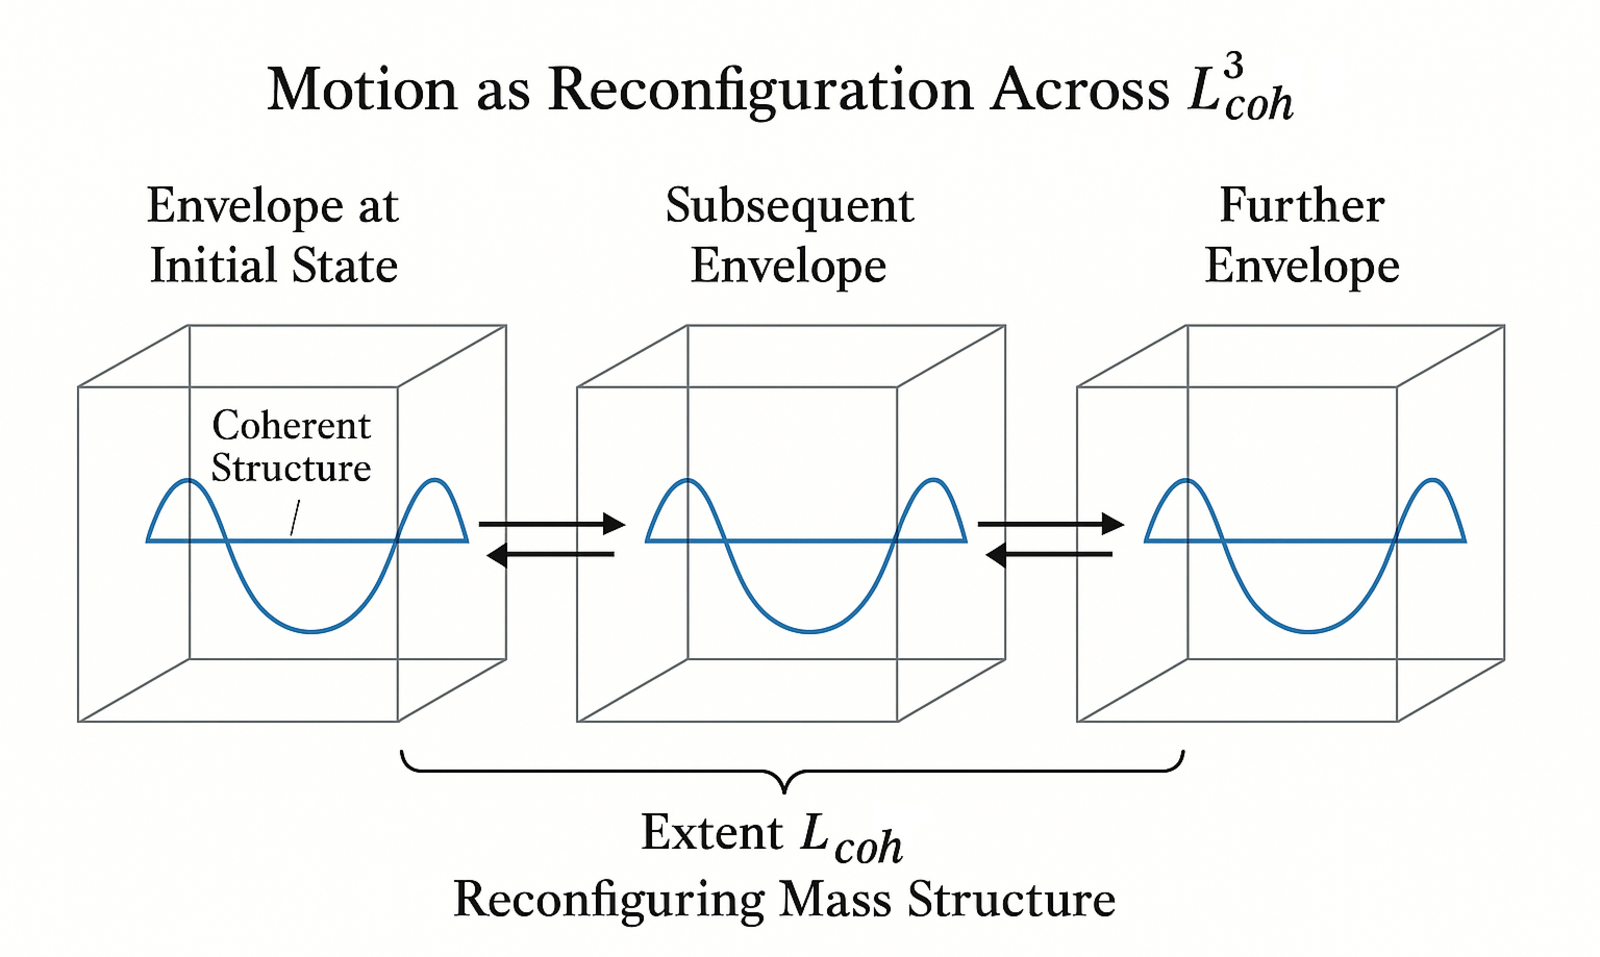
\includegraphics[width=0.85\textwidth]{figures/motion.pdf}
\caption{Motion as reconfiguration across coherence domains in QSD. A mass-phase structure persists by reconfiguring across adjacent \( L_{\text{coh}}^3 \) envelopes. No material translation occurs; instead, structural continuity is preserved under scalar pacing. Motion is reframed as a coherence-aligned causal process.}
\label{fig:motion}
\end{figure}

In this view, inertial motion is structurally equivalent to rest—it is a state of equilibrium where the coherence knot experiences no net tension imbalance and requires no energetic offload. Only acceleration introduces real substrate change: an attempt to reconfigure the mass-phase structure into a new geometric alignment. This reconfiguration demands scalar pacing and transverse emission, and thus constitutes a physical event. Acceleration is causally meaningful; uniform motion is not.

This coherence-bound view of motion also reframes a classical intuition: that two objects cannot occupy the same space and that motion requires a destination. In QSD, this principle is enforced structurally. A mass-phase configuration may only reconfigure into a new region of the substrate if that region has scalar-recovered, is below the collapse threshold, and can support coherent phase-locking. Motion therefore depends not only on internal readiness, but on the causal availability of the substrate into which it would move. This is conceptually analogous to classical mechanics, where motion into a lower-energy configuration or unoccupied phase space is required. However, in QSD, this constraint is not imposed statistically or geometrically—it is enforced dynamically by the substrate’s coherence pacing and recovery logic. Mass cannot move simply because it chooses to; it must wait until a structurally valid region of the substrate exists to receive it.

This interpretation explains the deep symmetry between rest and motion in relativistic physics. QSD shows that this symmetry arises not from observer equivalence, but from the structural neutrality of unchanged coherence. Motion is not transport—it is structural continuity. Stillness and uniform velocity are two forms of the same underlying equilibrium: coherence preserved across pacing cycles, undisturbed by collapse.


%%%%%%%%%%%%%%%%%%%%%%%%%%%%%%%%%%%%%%%%%%
\subsection{Unification and Substrate-Limited Physics}

Across classical mechanics, relativity, and quantum field theory, many foundational quantities—mass, time, quantization, inertia, radiation, and symmetry—are introduced as axioms or emergent abstractions. QSD offers a structural alternative: these phenomena are unified expressions of one physically bounded principle—the behavior of a Lorentz-invariant substrate governed by finite coherence, pacing, and causal offload capacity.

The coherence envelope \texorpdfstring{\( L_{\text{coh}}^3 \)}{Lcoh\^{}3} defines the minimal spatial region in which a complete, phase-locked, and causally admissible structure can exist. Within this envelope, quantized action arises not from imposed discreteness, but from the structural requirement that energy be serialized through scalar pacing. Planck’s constant \texorpdfstring{\( \hbar \)}{hbar} appears as a throughput limit on coherent offload; Planck energy \texorpdfstring{\( E_P \)}{Ep} as the envelope’s structural collapse threshold; and Planck time \texorpdfstring{\( t_P \)}{tP} as the scalar reset interval that gates all physical reconfiguration.

In this same coherence volume, radiation emerges not as spontaneous emission, but as the serialized release of internal waveform geometry—modulated by transverse propagation and paced by scalar collapse. Motion is reinterpreted as envelope-wise structural continuity, while acceleration becomes substrate reconfiguration. Inertia is not resistance to change—it is the substrate’s requirement that reconfiguration occur in full. Interference, likewise, is no longer cancellation by algebra, but the structural exclusion of incoherent configurations. And symmetry, rather than an assumed invariance, becomes the condition for waveform survival under scalar pacing and curvature balance, see Table \ref{fig:compare}.

What appears as disconnected rules in conventional physics are revealed in QSD to be surface expressions of a single structural logic: the substrate enforces causality through coherence-bound domains. Quantization, inertia, spectral discreteness, and conservation all follow from the same rule: only recoverable, pacing-aligned, curvature-balanced structures can exist, move, or interact.

This reframes physical law not as a system of imposed constraints, but as a reflection of what the substrate permits. The coherence envelope is not merely a length scale—it is the structural gate through which causal emergence becomes possible. In this view, physics is not written onto space. It is what survives in the substrate.

\begin{table}[H]
\centering
\caption{Comparison of Classical, QFT, and QSD Interpretations}
\label{fig:compare}
\begin{tabular}{|p{2.8cm}|p{3.5cm}|p{6.0cm}|}
\hline
\textbf{Phenomenon} & \textbf{Classical / QFT Interpretation} & \textbf{QSD Structural Interpretation} \\
\hline
Quantization & Imposed through operator algebra or energy levels & Arises from scalar-paced serialization and coherence geometry \\
\hline
Planck Constants & Empirically fixed, dimensional anchors & Derived from substrate throughput and envelope dynamics \\
\hline
Inertia & Resistance to force, quantified by \( F = ma \) & Cost of reconfiguring phase-locked structure across \( L_{\text{coh}}^3 \) \\
\hline
Motion & Continuous translation through space & Structural persistence across pacing cycles with no substrate displacement \\
\hline
Acceleration & Change in velocity, causes force or radiation & Causal reconfiguration event that disrupts scalar pacing and emits transverse energy \\
\hline
Spectral Lines & Quantum transitions between discrete energy levels & Serialized offload of internal waveform modes paced by scalar recovery \\
\hline
Symmetry & Invariance under transformation groups & Requirement for waveform closure and persistence within a coherence envelope \\
\hline
Interference & Amplitude cancellation of waves (superposition) & Structural exclusion of incoherent configurations that fail offload conditions \\
\hline
Energy & Quantified, conserved scalar property & Structured tension resolved through successful offload; only serialized energy is real \\
\hline
Fields & Continuous background entities supporting interactions & Secondary descriptions of structured propagation through the substrate medium \\
\hline
\end{tabular}
\end{table}


%%%%%%%%%%%%%%%%%%%%%%%%%%%%%%%%%%%%%%%%%%
\section*{Falsifiability and Outlook}

Although this paper presents a structural foundation for quantized behavior within the Quantum Substrate Dynamics (QSD) framework, it also suggests several avenues for empirical testing and further formal development.

The most direct testable implication concerns the serialized emission behavior predicted during the collapse of a mass-phase coherence knot. QSD predicts that such collapses produce not arbitrary energy dispersals, but structured spectral emissions whose frequency components reflect the internal waveform geometry of the original mass-phase configuration. This offers a falsifiable condition: high-resolution spectroscopy of coherent transitions—especially those involving metastable decay—should reveal spectral fingerprints that correlate with predicted envelope-supported modes. The spectrum should be serialized in a manner consistent with scalar pacing constraints and bounded by the transverse coherence speed \( c_t \).

Another potential point of falsification arises in the predicted phenomenon of inertial lag. QSD asserts that coherent mass-phase structures cannot be partially reconfigured and must transition between envelope-aligned configurations. This suggests a measurable delay between applied force and onset of acceleration for highly coherent systems, especially at small scales or in low-mass, high-purity test environments. Such effects may be accessible through precision accelerometry or ultra-cold matter systems.

QSD also reframes destructive interference as a structural coherence failure. This interpretation predicts that in experiments involving phase-inverted waveforms, such as optical or matter-wave interference, the absence of detection corresponds not to energy cancellation, but to causal exclusion: the superposed waveform cannot be serialized because it fails to meet the curvature and pacing requirements of the coherence envelope. Experiments designed to probe “which-path” indistinguishability, or to test energy accounting in null-detection regimes, may expose this offload gating mechanism.

The radial serialization model further predicts that particle-like emissions are structured projections of collapsing coherence geometry. Spectral emissions from radially symmetric offload events should not only reflect internal mode structure, but should arrive in time-resolved sequences that correspond to scalar pacing intervals. Ultrafast spectroscopic methods or time-resolved photon detection may be able to identify such serialized signatures, especially in highly coherent collapse contexts such as certain nuclear, atomic, or optical transitions.

In addition, QSD predicts the existence of a coherent momentum quantum—an irreducible impulse threshold required to initiate reconfiguration of a bound mass-phase knot. This implies that below a specific structural energy per envelope, no motion occurs, regardless of applied force. Systems approaching this limit may show thresholding behavior or quantized drag onset that differs from classical expectations.

Numerical predictions derived from QSD structure—such as the relation \[
 \hbar = \frac{c_t^4}{c_s} \cdot \frac{L_{\text{coh}}^2}{G} 
\] —can be compared to standard constants for dimensional consistency and structural fit. These relationships do not merely reproduce known values but aim to explain their origin from substrate geometry and coherence throughput.

Looking ahead, QSD invites formal extension. The envelope structure and scalar pacing logic presented here provide a foundation for coherence-aware equations of motion, interaction dynamics, and quantized evolution operators that respect the geometric and causal boundaries defined by \( L_{\text{coh}}^3 \). Future work will aim to formalize these dynamics and test the recoverable coherence model in both experimental and numerical regimes.




%%%%%%%%%%%%%%%%%%%%%%%%%%%%%%%%%%%%%%%%%%
\section{Conclusion}
%%%%%%%%%%%%%%%%%%%%%%%%%%%%%%%%%%%%%%%%%%
This paper has introduced the coherence envelope \texorpdfstring{\( L_{\text{coh}}^3 \)}{Lcoh\^{}3} as the fundamental structural unit of causality, quantization, and persistence within the Quantum Substrate Dynamics (QSD) framework. Unlike point-like models of matter or spacetime, the coherence envelope defines a finite, irreducible region in which phase-locked configurations may exist, reconfigure, and emit in accordance with scalar pacing and transverse propagation limits.

We have shown that Planck’s constant, energy, and time emerge as natural consequences of the envelope’s structural behavior: \texorpdfstring{\( \hbar \)}{hbar} arises from coherent offload throughput; \texorpdfstring{\( E_P \)}{Ep} from energy saturation limits; and \texorpdfstring{\( t_P \)}{tP} from scalar recovery intervals. Mass, in this context, is not an intrinsic property but a coherence knot stabilized within an envelope, with inertia arising from the cost of reconfiguration across envelope boundaries. Spectral emissions are revealed as serialized projections of internal waveform geometry, and symmetry emerges as the requirement for persistence within a bounded coherence domain.

These results suggest that much of what is traditionally accepted as fundamental in physics—quantization, inertia, field behavior, symmetry—can instead be understood as emergent from a deeper, structural limit condition. The coherence envelope is not a metaphor, but a physical threshold: the minimum support structure for reality to exist coherently. It is from this region that time, mass, motion, and information arise—not from abstract rules, but from the substrate’s own geometry.

%%%%%%%%%%%%%%%%%%%%%%%%%%%%%%%%%%%%%%%%%%
\vspace{6pt} 

%%%%%%%%%%%%%%%%%%%%%%%%%%%%%%%%%%%%%%%%%%
%% optional
%\supplementary{The following supporting information can be downloaded at:  \linksupplementary{s1}, Figure S1: title; Table S1: title; Video S1: title.}

% Only for journal Methods and Protocols:
% If you wish to submit a video article, please do so with any other supplementary material.
% \supplementary{The following supporting information can be downloaded at: \linksupplementary{s1}, Figure S1: title; Table S1: title; Video S1: title. A supporting video article is available at doi: link.}

% Only used for preprtints:
% \supplementary{The following supporting information can be downloaded at the website of this paper posted on \href{https://www.preprints.org/}{Preprints.org}.}

% Only for journal Hardware:
% If you wish to submit a video article, please do so with any other supplementary material.
% \supplementary{The following supporting information can be downloaded at: \linksupplementary{s1}, Figure S1: title; Table S1: title; Video S1: title.\vspace{6pt}\\
%\begin{tabularx}{\textwidth}{lll}
%\toprule
%\textbf{Name} & \textbf{Type} & \textbf{Description} \\
%\midrule
%S1 & Python script (.py) & Script of python source code used in XX \\
%S2 & Text (.txt) & Script of modelling code used to make Figure X \\
%S3 & Text (.txt) & Raw data from experiment X \\
%S4 & Video (.mp4) & Video demonstrating the hardware in use \\
%... & ... & ... \\
%\bottomrule
%\end{tabularx}
%}

\section*{Statements and Declarations}
\subsection*{Funding}  
The author received no financial support for the research, authorship, or publication of this article.
The author has no relevant financial or non-financial interests to disclose.

\subsection*{Competing Interests}  
The author declares no competing interests.

\subsection*{Author Contributions}  
The author solely conceived, developed, and wrote the manuscript, including all theoretical content, references, and formatting.

\subsection*{Data Availability}  
No datasets were generated or analyzed during the current study. All references are publicly available.

\subsection*{Ethical Approval}  
Not applicable.


%%%%%%%%%%%%%%%%%%%%%%%%%%%%%%%%%%%%%%%%%%
%% Optional

%% Only for journal Encyclopedia
%\entrylink{The Link to this entry published on the encyclopedia platform.}
\abbreviations{Abbreviations}{
The following abbreviations and symbols are used in this manuscript:
\\
\noindent
\begin{tabular}{@{}ll}
QSD   & Quantum Substrate Dynamics \\
\( L_{\text{coh}} \) & Coherence length (minimum spatial scale for offload) \\
\( L_{\text{coh}}^3 \) & Coherence envelope volume (minimum support for mass-phase knot) \\
\( c_s \) & Scalar coherence recovery speed (temporal pacing mode) \\
\( c_t \) & Transverse coherence propagation speed (spatial mode) \\
\( t_P \) & Planck time (scalar recovery interval: \( L_{\text{coh}} / c_s \)) \\
\( E_P \) & Planck energy (collapse threshold: \( c_t^4 / G \cdot L_{\text{coh}} \)) \\
\( \hbar \) & Reduced Planck constant (derived substrate offload unit) \\
\( \Phi(x,t) \) & Coherence configuration (proto-field representation) \\
GPS  & Global Positioning System \\
SR   & Special Relativity \\
GR   & General Relativity \\
\end{tabular}
}




%%%%%%%%%%%%%%%%%%%%%%%%%%%%%%%%%%%%%%%%%%
%% Optional
\appendixtitles{no} % Leave argument "no" if all appendix headings stay EMPTY (then no dot is printed after "Appendix A"). If the appendix sections contain a heading then change the argument to "yes".
\appendixstart
\appendix
%%%%%%%%%%%%%%%%%%%%%%%%%%%%%%%%%%%%%%%%%%%%%%%
\section[\appendixname~\thesection]{}
\subsection[\appendixname~\thesubsection]{Substrate Geometry, Timing, and the Modeling of Inertial Motion}
%%%%%%%%%%%%%%%%%%%%%%%%%%%%%%%%%%%%%%%%%%%%%%
\subsubsection{Motivation}
Conventional models treat uniform motion as a symmetry state—either a straight-line path in a geometric manifold (special relativity) or a constant phase solution in a linear field (quantum mechanics). These models describe motion without explaining its physical basis. QSD, by contrast, defines uniform motion structurally: as the unbroken persistence of a phase-locked mass configuration across a sequence of coherent envelopes.

\subsubsection{Geometry and Causal Persistence}

In QSD, the substrate is stationary and causal structure is governed by transitions between discrete coherence volumes of size \texorpdfstring{\( L_{\text{coh}}^3 \)}{Lcoh\^{}3}. A mass-phase structure in uniform motion is one that maintains phase stability and scalar pacing alignment across these volumes without initiating reconfiguration. No collapse occurs, and therefore no causal event is registered in the substrate. Uniform motion is modeled not by position change, but by the absence of structural disruption.

\subsubsection{Timing and Scalar Recovery Constraints}

Scalar pacing sets a temporal constraint on how frequently an envelope may undergo reconfiguration:
\[
t_P = \frac{L_{\text{coh}}}{c_s}.
\]
For motion to appear uniform, coherence transitions must either:
\begin{itemize}
    \item Not occur at all (i.e., perfect structural persistence), or
    \item Occur in a perfectly synchronized, pacing-compliant sequence.
\end{itemize}
This scalar-timed condition replaces arbitrary coordinate transformations with physically enforceable coherence continuity.

\subsubsection{Toward a Formal Model}

Although a full operator framework remains for future work, the substrate imposes constraints that could be formalized dynamically:
\[
\Phi(x,t) = \Phi_0(x - v t) \quad \text{with} \quad \frac{d\Phi}{dt} = 0 \quad \text{in each } L_{\text{coh}}^3.
\]
Here, \texorpdfstring{\( \Phi \)}{Phi} represents a coherence-preserving field configuration moving uniformly through the substrate by virtue of unbroken structure, not transport. Motion becomes a map of phase persistence across a causal coherence grid.

\subsubsection{Implications}

This structural reinterpretation provides a pathway to model uniform motion, transitions, and inertial frame equivalence not as imposed symmetries, but as outcomes of recoverable substrate geometry. It offers the potential to extend classical and quantum equations of motion into nonlinear, structure-aware coherence dynamics, grounded in physical substrate behavior.

%%%%%%%%%%%%%%%%%%%%%%%%%%%%%%%%%%%%%%%%%%%%%%%
\section[\appendixname~\thesection]{}
\subsection[\appendixname~\thesubsection]{Coherent Momentum Quantum and Structural Complexity}
%%%%%%%%%%%%%%%%%%%%%%%%%%%%%%%%%%%%%%%%%%%%%%%
%\subsubsection{SUB B}
\label{app:coherent-momentum-quantum}
In QSD, inertial motion is reinterpreted not as continuous translation but as a reconfiguration of phase-locked coherence across substrate boundaries. As established in Section \ref{sec:coherent-momentum-quantum} movement requires full reconfiguration of each occupied \texorpdfstring{\( L_{\text{coh}}^3 \)}{Lcoh\^{}3} envelope. No partial offload is permitted. This introduces a minimum energetic cost per motion event and implies the existence of a quantized impulse threshold: the \textit{coherent momentum quantum}.

We define the coherent momentum quantum, \texorpdfstring{\( p_q \)}{pq}, as the minimum impulse required to initiate substrate-compliant reconfiguration of a mass-phase structure. Unlike classical momentum, which varies continuously with velocity, \texorpdfstring{\( p_q \)}{pq} is an envelope-scale quantity, constrained by the structure's internal complexity, curvature, and tension profile.

We propose the following structural model:
\[
p_q = \kappa \cdot \frac{h}{L_{\text{coh}}}
\]
where:
\begin{itemize}
    \item \( h \) is Planck’s constant,
    \item \( L_{\text{coh}} \) is the coherence envelope length scale,
    \item \( \kappa \geq 1 \) is a dimensionless \textit{coherence complexity factor}.
\end{itemize}

The factor \( \kappa \) encodes structural details of the mass-phase waveform and may depend on:
\begin{enumerate}
    \item The number of coupled \texorpdfstring{\( L_{\text{coh}}^3 \)}{Lcoh\^{}3} volumes,
    \item The internal curvature density of the waveform (e.g., via \texorpdfstring{\( \int |\nabla^2 \phi|^2 d^3x \)}{∫|∇²ϕ|²}),
    \item The number of standing modes, phase folds, or topological nodes.
\end{enumerate}

For simple, symmetric coherence knots (e.g., idealized spherical masses), \( \kappa \approx 1 \) may apply. For complex or extended structures, \( \kappa \) increases, reflecting a higher substrate reconfiguration cost. This scaling provides a natural mechanism for inertial variation among structures of equal mass but differing internal coherence geometry.

This model offers several testable predictions. Systems with greater waveform complexity should exhibit larger minimum impulse thresholds and stronger inertial lag under acceleration. It also suggests that motion, at its most fundamental level, may be discretized—not by mathematical quantization, but by substrate-enforced coherence limits.

Future work may formalize \( \kappa \) from first principles or derive it from observed spectral structures, establishing a link between measurable emissions and internal inertial geometry. The coherent momentum quantum may serve as a foundational quantity in any full dynamical formulation of QSD motion.


%%%%%%%%%%%%%%%%%%%%%%%%%%%%%%%%%%%%%%%%%%
%\isPreprints{} % If the paper is ``preprints'', please uncomment this parenthesis.
%\printendnotes[custom] % Un-comment to print a list of endnotes

\reftitle{References}

% Please provide either the correct journal abbreviation (e.g. according to the “List of Title Word Abbreviations” http://www.issn.org/services/online-services/access-to-the-ltwa/) or the full name of the journal.
% Citations and References in Supplementary files are permitted provided that they also appear in the reference list here. 

%=====================================
% References, variant A: external bibliography
%=====================================
% \bibliography{your_external_BibTeX_file}

%=====================================
% References, variant B: internal bibliography
%=====================================


% ACS format
\isAPAandChicago{}{%
\begin{thebibliography}{999}
% Reference 
\bibitem{bush2025}
\textbf{Preprint.} Bush, M. (2025). Quantum Substrate Dynamics (QSD): A Relativistic Field Model of Emergent Mass, Inertia and Gravity. \textit{Preprints}, 2025060988. \url{https://doi.org/10.20944/preprints202506.0988.v1}
% Reference
\bibitem{bush-planck-2025}
\textbf{Preprint.} Bush, M. (2025). Planck’s Constant Physically Derived Through Quantum Substrate Dynamics: A Mode-Ratio and Offload-Based Origin for Quantization and Temporal Structure. \textit{Preprints}, 2024010211. \url{https://doi.org/10.20944/preprints202401.0211.v1}
% Reference
\bibitem{bush-timedilation-2025}
\textbf{Preprint.} Bush, M. (2025). Time Dilation from Quantum Substrate Dynamics: A Coherence-Based Origin for Relativistic Delay. \textit{Preprints}, 2025062144. \url{https://doi.org/10.20944/preprints202506.2144.v1}
% Reference 
\bibitem{planck1901}
\textbf{Journal article.} Planck, M. (1901). On the Law of Distribution of Energy in the Normal Spectrum. \textit{Annalen der Physik}, 4(553–563). \url{https://doi.org/10.1002/andp.19053221004} 
% Reference 
\bibitem{einstein1905} 
\textbf{Journal article.} Einstein, A. (1905). On the electrodynamics of moving bodies. \textit{Annalen der Physik}, 322(10), 891–921. 
\url{https://doi.org/10.1002/andp.19053221008}
% Reference 
\bibitem{einstein1915} 
\textbf{Journal article.} Einstein, A. (1915). The field equations of gravitation. \textit{Sitzungsberichte der Preussischen Akademie der Wissenschaften}.
% Reference 
\bibitem{ashby-gps}
Ashby, N. Relativity in the Global Positioning System. {\em Living Rev. Relativ.} {\bf 2003}, {\em 6}, 1--50. \url{https://doi.org/10.12942/lrr-2003-1}.
% Reference
\bibitem{bailey-muon}
Bailey, J.; Borer, K.; Combley, F.; Drumm, H.; Krienen, F.; Picasso, E.; von Ruden, W.; Farley, F.J.M.; Field, J.H. Measurements of relativistic time dilatation for positive and negative muons in a circular orbit. {\em Nature} {\bf 1977}, {\em 268}, 301--305. \url{https://doi.org/10.1038/268301a0}.
% Reference
\bibitem{peskin1995}
Peskin, M. E., \& Schroeder, D. V. (1995). \textit{An Introduction to Quantum Field Theory}. Addison-Wesley.
% Reference
\bibitem{weinberg1995}
Weinberg, S. (1995). \textit{The Quantum Theory of Fields, Volume 1: Foundations}. Cambridge University Press.
% Reference
\bibitem{ryder1996}
Ryder, L. H. (1996). \textit{Quantum Field Theory} (2nd ed.). Cambridge University Press.
% Reference
\bibitem{amelino1994}
Amelino-Camelia, G. (1994). Limits on the measurability of space-time distances in the semiclassical approximation of quantum gravity. \textit{Modern Physics Letters A}, \textbf{9}(41), 3415–3422.
% Reference
\bibitem{garay1995}
Garay, L. J. (1995). Quantum gravity and minimum length. \textit{International Journal of Modern Physics A}, \textbf{10}(2), 145–165.
% Reference
\bibitem{volovik2003}
Volovik, G. E. (2003). \textit{The Universe in a Helium Droplet}. Oxford University Press.
% Reference
\bibitem{barcelo2005}
Barceló, C., Liberati, S., \& Visser, M. (2005). Analogue gravity. \textit{Living Reviews in Relativity}, \textbf{8}(12), 1–112.
% Reference
\bibitem{griffiths1995}
Griffiths, D. J. (1995). \textit{Introduction to Quantum Mechanics}. Prentice Hall.
% Reference
\bibitem{peskin1995}
Peskin, M. E., \& Schroeder, D. V. (1995). \textit{An Introduction to Quantum Field Theory}. Addison-Wesley.
% Reference
\bibitem{loudon2000}
Loudon, R. (2000). \textit{The Quantum Theory of Light} (3rd ed.). Oxford University Press.
%reference
\bibitem{feynman-qed}
Feynman, R.P.; Leighton, R.B.; Sands, M. \textit{The Feynman Lectures on Physics, Vol. 3: Quantum Mechanics}; Addison-Wesley: Reading, MA, USA, 1965. \url{https://www.feynmanlectures.caltech.edu/III_toc.html}
\end{thebibliography}
}


% Chicago format (Used for journal: arts, genealogy, histories, humanities, jintelligence, laws, literature, religions, risks, socsci)
\isChicagoStyle{%
\begin{thebibliography}{999}
% Reference 1
%\bibitem[Aranceta-Bartrina(1999a)]{ref-journal}
%Aranceta-Bartrina, Javier. 1999a. Title of the cited article. \textit{Journal Title} %6: 100--10.
% Reference 2

\end{thebibliography}
}{}

% APA format (Used for journal: admsci, behavsci, businesses, econometrics, economies, education, ejihpe, games, humans, ijfs, journalmedia, jrfm, languages, psycholint, publications, tourismhosp, youth)
\isAPAStyle{%
\begin{thebibliography}{999}
% Reference 1
%\bibitem[\protect\citeauthoryear{Azikiwe \BBA\ Bello}{{2020a}}]{ref-journal}
%Azikiwe, H., \& Bello, A. (2020a). Title of the cited article. \textit{Journal Title}, \textit{Volume}(Issue), 
%Firstpage--Lastpage/Article Number.

\end{thebibliography}
}{}

% If authors have biography, please use the format below
%\section*{Short Biography of Authors}
%\bio
%{\raisebox{-0.35cm}{\includegraphics[width=3.5cm,height=5.3cm,clip,keepaspectratio]{Definitions/author1.pdf}}}
%{\textbf{Firstname Lastname} Biography of first author}
%
%\bio
%{\raisebox{-0.35cm}{\includegraphics[width=3.5cm,height=5.3cm,clip,keepaspectratio]{Definitions/author2.jpg}}}
%{\textbf{Firstname Lastname} Biography of second author}

% For the MDPI journals use author-date citation, please follow the formatting guidelines on http://www.mdpi.com/authors/references
% To cite two works by the same author: \citeauthor{ref-journal-1a} (\citeyear{ref-journal-1a}, \citeyear{ref-journal-1b}). This produces: Whittaker (1967, 1975)
% To cite two works by the same author with specific pages: \citeauthor{ref-journal-3a} (\citeyear{ref-journal-3a}, p. 328; \citeyear{ref-journal-3b}, p.475). This produces: Wong (1999, p. 328; 2000, p. 475)

%%%%%%%%%%%%%%%%%%%%%%%%%%%%%%%%%%%%%%%%%%
%% for journal Sci
%\reviewreports{\\
%Reviewer 1 comments and authors’ response\\
%Reviewer 2 comments and authors’ response\\
%Reviewer 3 comments and authors’ response
%}
%%%%%%%%%%%%%%%%%%%%%%%%%%%%%%%%%%%%%%%%%%
\PublishersNote{}
%\isPreprints{} % If the paper is ``preprints'', please uncomment this parenthesis.
\end{document}

